\chapter{Information retrieval and web search}
\emph{Information retrieval} of kortweg IR is een reeks van technieken die gebruikt worden om tekst te bewerken voordat deze gebruikt worden in data mining algoritmes. IR helpt gebruikers met behulp van \emph{queries} zodat deze informatie kunnen bijwinnen. Algemeen definieert men IR dus als de studie die de verzameling, verwerking, opslag en verspreiding van informatie mogelijk maakt.

Architecturaal kan men IR als volgt voorstellen:
\begin{figure}
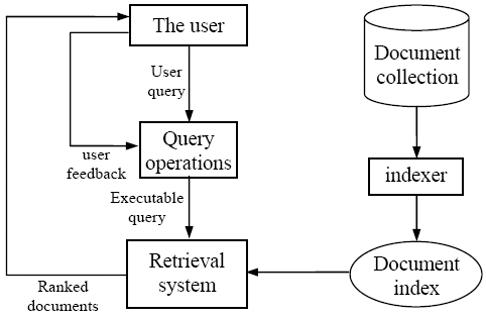
\includegraphics[width=0.8\textwidth]{res/IR}
\caption{De architectuur van IR.}
\end{figure}

Hierbij kan de gebruiker dus aan de hand van query's informatie opvragen. Gebaseerd op het document dat hij hierbij terugkrijgt kan de query dan eventueel aangepast worden. Er zijn verschillende soorten query's mogelijk:
\begin{itemize}
\item \textbf{Keyword queries}: Zoeken met kernwoorden zoals bijvoorbeeld op Google.
\item \textbf{Boolean queries}: AND, OR, NOT gebruiken om query's samen te stellen.
\item \textbf{Phrase queries}: Zoeken via zinnen.
\item \textbf{Proximity queries}: Zoeken naar woorden die normaal gezien vaak samen voorkomen.
\item \textbf{Full document queries}: Gebruikt bij bijvoorbeeld plagiaatcontrole.
\item \textbf{Natural language questions}: Gebruikt bij \emph{voice assistants} zoals Siri, Cortana, Alexa \dots
\end{itemize}

Een IR model bepaalt hoe een document en een query zijn opgebouwd. De meest voorkomende zijn booleaanse modellen, \emph{vector spac}e modellen en \emph{statistical language} modellen.
\section{Booleaans model}
Bij een booleaans model wordt elk document en elke query beschouwd als een groep van woorden. De volgorde waarin deze voorkomen is niet belangrijk.
Algemeen stellen we dat voor een groep documenten $D$ we $V = \{ t_1, t_2, ..., t_{|V|}\}$ defini\"eren als de woordenschat van deze documenten. 
Aan elk woord $t_i$ uit document $d_j \in D$ wordt een gewicht $w_{ij} = 1$ toegekend. Voor termen die niet voorkomen in document $d_j$ is het gewicht gelijk aan nul. Het document is dus gelijk aan: 

\begin{equation}
d_j = \left( w_{1j},w_{2j},..,w_{|V|j} \right)
\end{equation}

Met behulp van booleaanse operatoren kunnen query's op opgebouwd worden; waarbij het gewicht $w_{ij}$ in beschouwing wordt genomen. Ieder document waarvoor het resultaat \emph{true} is, wordt opgehaald en teruggegeven. De resultaten voor deze query's zijn vaak slecht omdat er geen rekening wordt gehouden met de frequentie van woorden. De gewichten zijn immers 0 of 1. Een voorbeeld van zo een query: (\emph{voetbal} AND (NOT \emph{anderlecht})).

\section{Vector space model}
Bij een \emph{vector space model} of VSM wordt een document opnieuw voorgesteld als een groep van woorden. Elk document is een vector met daarin per woord een gewicht. In tegenstelling tot bij het booleaans model is het gewicht niet gewoon 0 of 1. Om dit gewicht te berekenen maken we gebruik van een \emph{Term Frequency} (TF) model. De definitie  hiervan is eenvoudig; het gewicht van een term $t_i$ in een document $d_j$ is het aantal keren dat $t_i$ voorkomt in $d_j$ voorgesteld in $f_{ij}$. We kunnen deze waarden ook normaliseren. We spreken dan van TF-IDF model. IDF staat voor \emph{Inverse Document Frequency}. De gewichten bij TF-IDF worden dan als volgt berekend:
\begin{equation}
tf_{ij} = \frac{f_{ij}}{max_{f_j \in d_j}f_j}
\end{equation}
Met $N$ het aantal documenten en $df_i$ het aantal documenten dat $t_i$ bevat:
\begin{equation}
idf_i = \log{ \frac{N}{df_i}}
\end{equation}
Wordt het gewicht:
\begin{equation}
w_{ij} = tf_{ij} \cdot idf_i
\end{equation}
We houden dus niet alleen rekening met de frequentie van een woord in 1 document, maar kijken over alle documenten heen.

Het opstellen van een query is bij VSM is minder eenvoudig dan bij een booleaans model en maakt gebruik van een inwendig product (dot product) tussen 2 vectoren. We stellen immers zowel de query  als het document voor als een vector. Hoe beter de vectoren overeenkomen, hoe groter de cosinus tussen deze vectoren. Algemeen berekenen we de overeenkomst als

\begin{equation}
\cos{\left(d_j,q\right)} = \frac{d_j \cdot q}{||d_j|| ||q||} =
\frac{\sum_{i=1}^{|V|}{w_{ij} w_{iq}}}{\sqrt[]{
\sum_{i=1}^{|V|}{ w_{ij}^2}
\sum_{i=1}^{|V|}{w_{iq}^2}
}}
\end{equation}

%
\paragraph{Voorbeeld}

Stel dat we volgende woordenschat hebben: \emph{hardware,software,users} en volgende set van documenten met als query: 'hardware and software':

\begin{table}[h]
\centering
\caption{Een verzameling met applicaties $D$.}
\label{tabel:sl_ex1}
\begin{tabular}{c|c}
\textbf{Set} & \textbf{Inhoud} \\
$A_1$ & $\{1,0,0\}$ \\
$A_2$ & $\{0,1,0\}$ \\
$A_3$ & $\{0,0,1\}$ \\
$A_4$ & $\{1,1,0\}$ \\
$A_5$ & $\{1,0,1\}$ \\
$A_6$ & $\{0,1,1\}$ \\
$A_7$ & $\{1,1,1\}$ \\
$A_8$ & $\{1,0,1\}$ \\
$A_9$ & $\{0,1,1\}$
\end{tabular}
\end{table}
%

Bij het booleaanse model krijgen we dan $A_4$ en $A_7$ terug. We kijken immers gewoon of de term voorkomt en gebruiken een AND-relatie. 

Bij VSM berekenen we telkens de cosinus tussen de twee vectoren. De query---voorgesteld als vector---ziet er als volgt uit: 
\begin{equation}
q(1,1,0)
\end{equation}

We krijgen de volgende waarden per document:

\begin{table}[h]
\centering
\caption{Een verzameling met applicaties $D$.}
\label{tabel:sl_ex1}
\begin{tabular}{c|c|c}
\textbf{Set} & \textbf{Inhoud} & \textbf{cos} \\
$A_1$ & $\{1,0,0\}$ & 0,71 \\
$A_2$ & $\{0,1,0\}$ & 0,71\\
$A_3$ & $\{0,0,1\}$ & 0\\
$A_4$ & $\{1,1,0\}$ & 1\\
$A_5$ & $\{1,0,1\}$ & 0,5\\
$A_6$ & $\{0,1,1\}$ & 0,5\\
$A_7$ & $\{1,1,1\}$ & 0,82\\
$A_8$ & $\{1,0,1\}$ & 0,5\\
$A_9$ & $\{0,1,1\}$ & 0,5\\
\end{tabular}
\end{table}

Hieruit krijgen we dan de volgende documenten terug: $A_1,A_2,A_4,A_5,A_6,A_7,A_8,A_9$.

\section{Text processing}
Indien we het huidig model zouden gebruiken, dan zou dit geen goede resultaten geven. Documenten bevatten vaak woorden die geen waarde toevoegen: stopwoorden. Het verwijderen van deze stopwoorden verhoogt de effici\"entie en accuraatheid van het zoeksysteem. Men kan lijsten met stopwoorden online vinden. Voor sommige toepassingen wordt bovenop deze lijst nog een extra reeks woorden toegevoegd die men ook als stopwoorden beschouwd. 

Naast stopwoorden moet men ook nog \emph{stemming} toepassen, waarmee herleid wordt naar de stam van een woord. Woorden zoals loop, loper, loopt, gelopen \dots zijn kleine veranderingen op het woord loop. \emph{Stemming} maakt het mogelijk om dit allemaal terug te laten wijzen op hetzelfde basiswoord. Ook hier is het doel om de effici\"entie te verhogen en de grootte van de index te verkleinen. Per taal is er een reeks technieken beschikbaar om aan \emph{stemming} te doen. Zo kan men in het Engels bij woorden die op -ing eindigen, dit laatste wegdoen.

Tot slot kan men opnieuw TF-IDF toepassen om de termen bij te houden in de index.

Zoals gezien zijn er meerdere methoden om op queries te reageren. We hebben dus een manier nodig om deze te evalueren. Hierbij stellen we ons 2 vragen:
\begin{itemize}
\item Is elke opgehaald document relevant?
\item Zijn alle relevante documenten opgehaald?
\end{itemize}
De eerste vraag heeft betrekking tot de nauwkeurigheid van de zoekopdracht, terwijl de tweede betrekking heeft op de volledigheid. Dit wordt duidelijk gemaakt in de volgende figuur:

\begin{figure}[h]
\centering
\caption{Nauwkeurigheid en volledigheid van een zoekopdracht.}
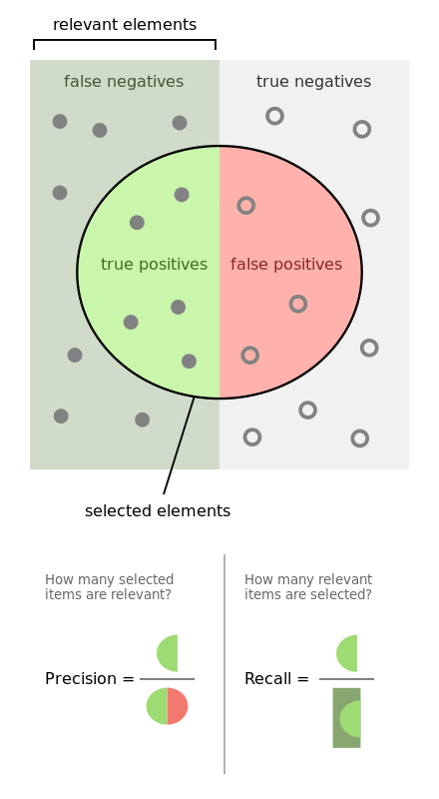
\includegraphics[width=0.55\textwidth]{res/evaluation_queries}
\end{figure}

\newpage
We kunnen deze algoritmes met elkaar vergelijken met de volgende formule; waarmee we dan grafieken kunnen opstellen om de verschillende algoritmes visueel met elkaar te vergelijken.

\begin{equation}
\overline{p}\left(r_i\right)=\frac{1}{|Q|}\sum_{j=1}^{|Q|}{p_j(r_i)}
\end{equation}

%
\subsection{Inverted index}
Men kan een zoekopdracht via het internet beschouwen als een groot IR systeem. Hierbij moet een \emph{webcrawler} alle webpagina's die deze tegenkomt opslaan in wat men een ge\"inverteerde indexing database noemt.
Voor ieder item kan een lijst met documenten worden bijgehouden waar het item in voorkomt. Dit is een ge\"inverteerde index, wat als voordeel heeft dat het vinden van documenten in vaste tijdsduur kan gebeuren. Daarnaast kunnen meerdere query-elementen ook eenvoudig verwerkt worden.

Als we een query $q$ beschouwen, dan omvat zoeken de volgende stappen:

\begin{enumerate}
\item \textbf{Vocabulary search}: Zoek alle woorden in $q$ in de ge\"inverteerde index.
\item \textbf{Resultaten mergen}: \emph{Merge} de resulaten die alle of enkele woorden uit $q$ bevatten.
\item \textbf{Rank score computation}: Order de documenten.
\end{enumerate}

